\let\negmedspace\undefined
\let\negthickspace\undefined
\documentclass[journal]{IEEEtran}
\usepackage[a4paper, margin=10mm, onecolumn]{geometry}
%\usepackage{lmodern} % Ensure lmodern is loaded for pdflatex
\usepackage{tfrupee} % Include tfrupee package

\setlength{\headheight}{1cm} % Set the height of the header box
\setlength{\headsep}{0mm}  % Set the distance between the header box and the top of the text

\usepackage{gvv-book}
\usepackage{gvv}
\usepackage{cite}
\usepackage{amsmath,amssymb,amsfonts,amsthm}
\usepackage{algorithmic}
\usepackage{graphicx}
\usepackage{float}
\usepackage{textcomp}
\usepackage{xcolor}
\usepackage{txfonts}
\usepackage{listings}
\usepackage{enumitem}
\usepackage{mathtools}
\usepackage{gensymb}
\usepackage{comment}
\usepackage[breaklinks=true]{hyperref}
\usepackage{tkz-euclide} 
\usepackage{listings}
% \usepackage{gvv}                                        
\def\inputGnumericTable{}                                 
\usepackage[latin1]{inputenc}                                
\usepackage{color}                                            
\usepackage{array}                                            
\usepackage{longtable}                                       
\usepackage{calc}                                             
\usepackage{multirow}                                         
\usepackage{hhline}                                           
\usepackage{ifthen}                                           
\usepackage{lscape}
\usepackage{tikz}
\usetikzlibrary{patterns}

\begin{document}

\bibliographystyle{IEEEtran}
\vspace{3cm}

\title{4.13.67}
\author{ee25btech11063-vejith}

\maketitle
% \maketitle
% \newpage
% \bigskip
{\let\newpage\relax\maketitle}
\renewcommand{\thefigure}{\theenumi}
\renewcommand{\thetable}{\theenumi}
\setlength{\intextsep}{10pt} % Space between text and floats
\textbf{Question}\\
The area of the triangle formed by the intersection of line parallel to X axis and passing through $\Vec{p}$(h,k) with the lines y=x and x+y=2 is 4h$^2$.Find the locus of point $\Vec{p}$\\
\textbf{Solution}:\\
line parallel to X axis is of the form 
\begin{align}
    \Vec{n}^T\Vec{x}=c.\\
     \implies \brak{0\hspace{0.5cm}1}\myvec{x\\y}=c.
\end{align}
As the above line passes through $\Vec{p}$(h,k)
\begin{align}
     \brak{0\hspace{0.5cm}1}\myvec{h\\k}=c.
     \implies c=k.
\end{align}
The three lines are as follows
\begin{align}
    y=k\implies \brak{0\hspace{0.5cm}1}\myvec{x\\y}=k.\\
    -x+y=0 \implies \brak{-1\hspace{0.5cm}1}\myvec{x\\y}=0.\\
    x+y=2 \implies\brak{1\hspace{0.5cm}1}\myvec{x\\y}=2.
\end{align}
Let $\Vec{A}$,$\Vec{B}$,$\Vec{C}$ be the point of intersection of above 3 lines\\
On solving equation (4) and (5)
\begin{align}
    \begin{pmatrix}
        0 & 1\\
        -1 & 1
    \end{pmatrix} \myvec{x\\y}=\myvec{k\\0}.\\
    \implies \vec{A}=\myvec{x\\y}=\myvec{k\\k}
\end{align}
On solving equation (5) and (6)
\begin{align}
    \begin{pmatrix}
        -1 & 1\\
        1 & 1
    \end{pmatrix} \myvec{x\\y}=\myvec{0\\2} &\xrightarrow{R_2 \leftrightarrow R_1+R_2} \begin{pmatrix}
        -1 & 1\\
        0 & 2
    \end{pmatrix} \myvec{x\\y}=\myvec{0\\2}.\\
 \implies \vec{B}=\myvec{x\\y}=\myvec{1\\1}
\end{align}
On solving equation (4) and (6)
\begin{align}
    \begin{pmatrix}
        0 & 1\\
        1 & 1
    \end{pmatrix} \myvec{x\\y}=\myvec{k\\2}.\\
    \implies \vec{C}=\myvec{x\\y}=\myvec{2-k\\k}
\end{align}
\begin{align}
    \text{area of }\triangle \text{ABc}=\frac{1}{2}\norm{(\vec{A}-\vec{B})\times(\vec{B}-\vec{C})}\\
    =\frac{1}{2}\norm{\myvec{k-1\\k-1}\times\myvec{k-1\\1-k}}\\
    =\frac{1}{2}(2(k-1)^2)=(k-1)^2.
\end{align}
Given area of the triangle formed by the intersection of above 3 lines is 4h$^2$.
\begin{align}
    \implies (k-1)^2= 4h^2.\\
    \implies (y-1)^2=4x^2\\
    \implies(y-1-2x)(y-1+2x)=0
    \end{align}
   $\implies$ The locus of $\vec{p}$ is pair of  straight lines
   \begin{align}
     y-1-2x=0. \implies  \brak{-2\hspace{0.5cm}1}\myvec{x\\y}=1.\\
     y-1+2x=0. \implies  \brak{2\hspace{0.5cm}1}\myvec{x\\y}=1.
   \end{align}
   \\ \\ 
   \begin{figure}[H]
    \centering
    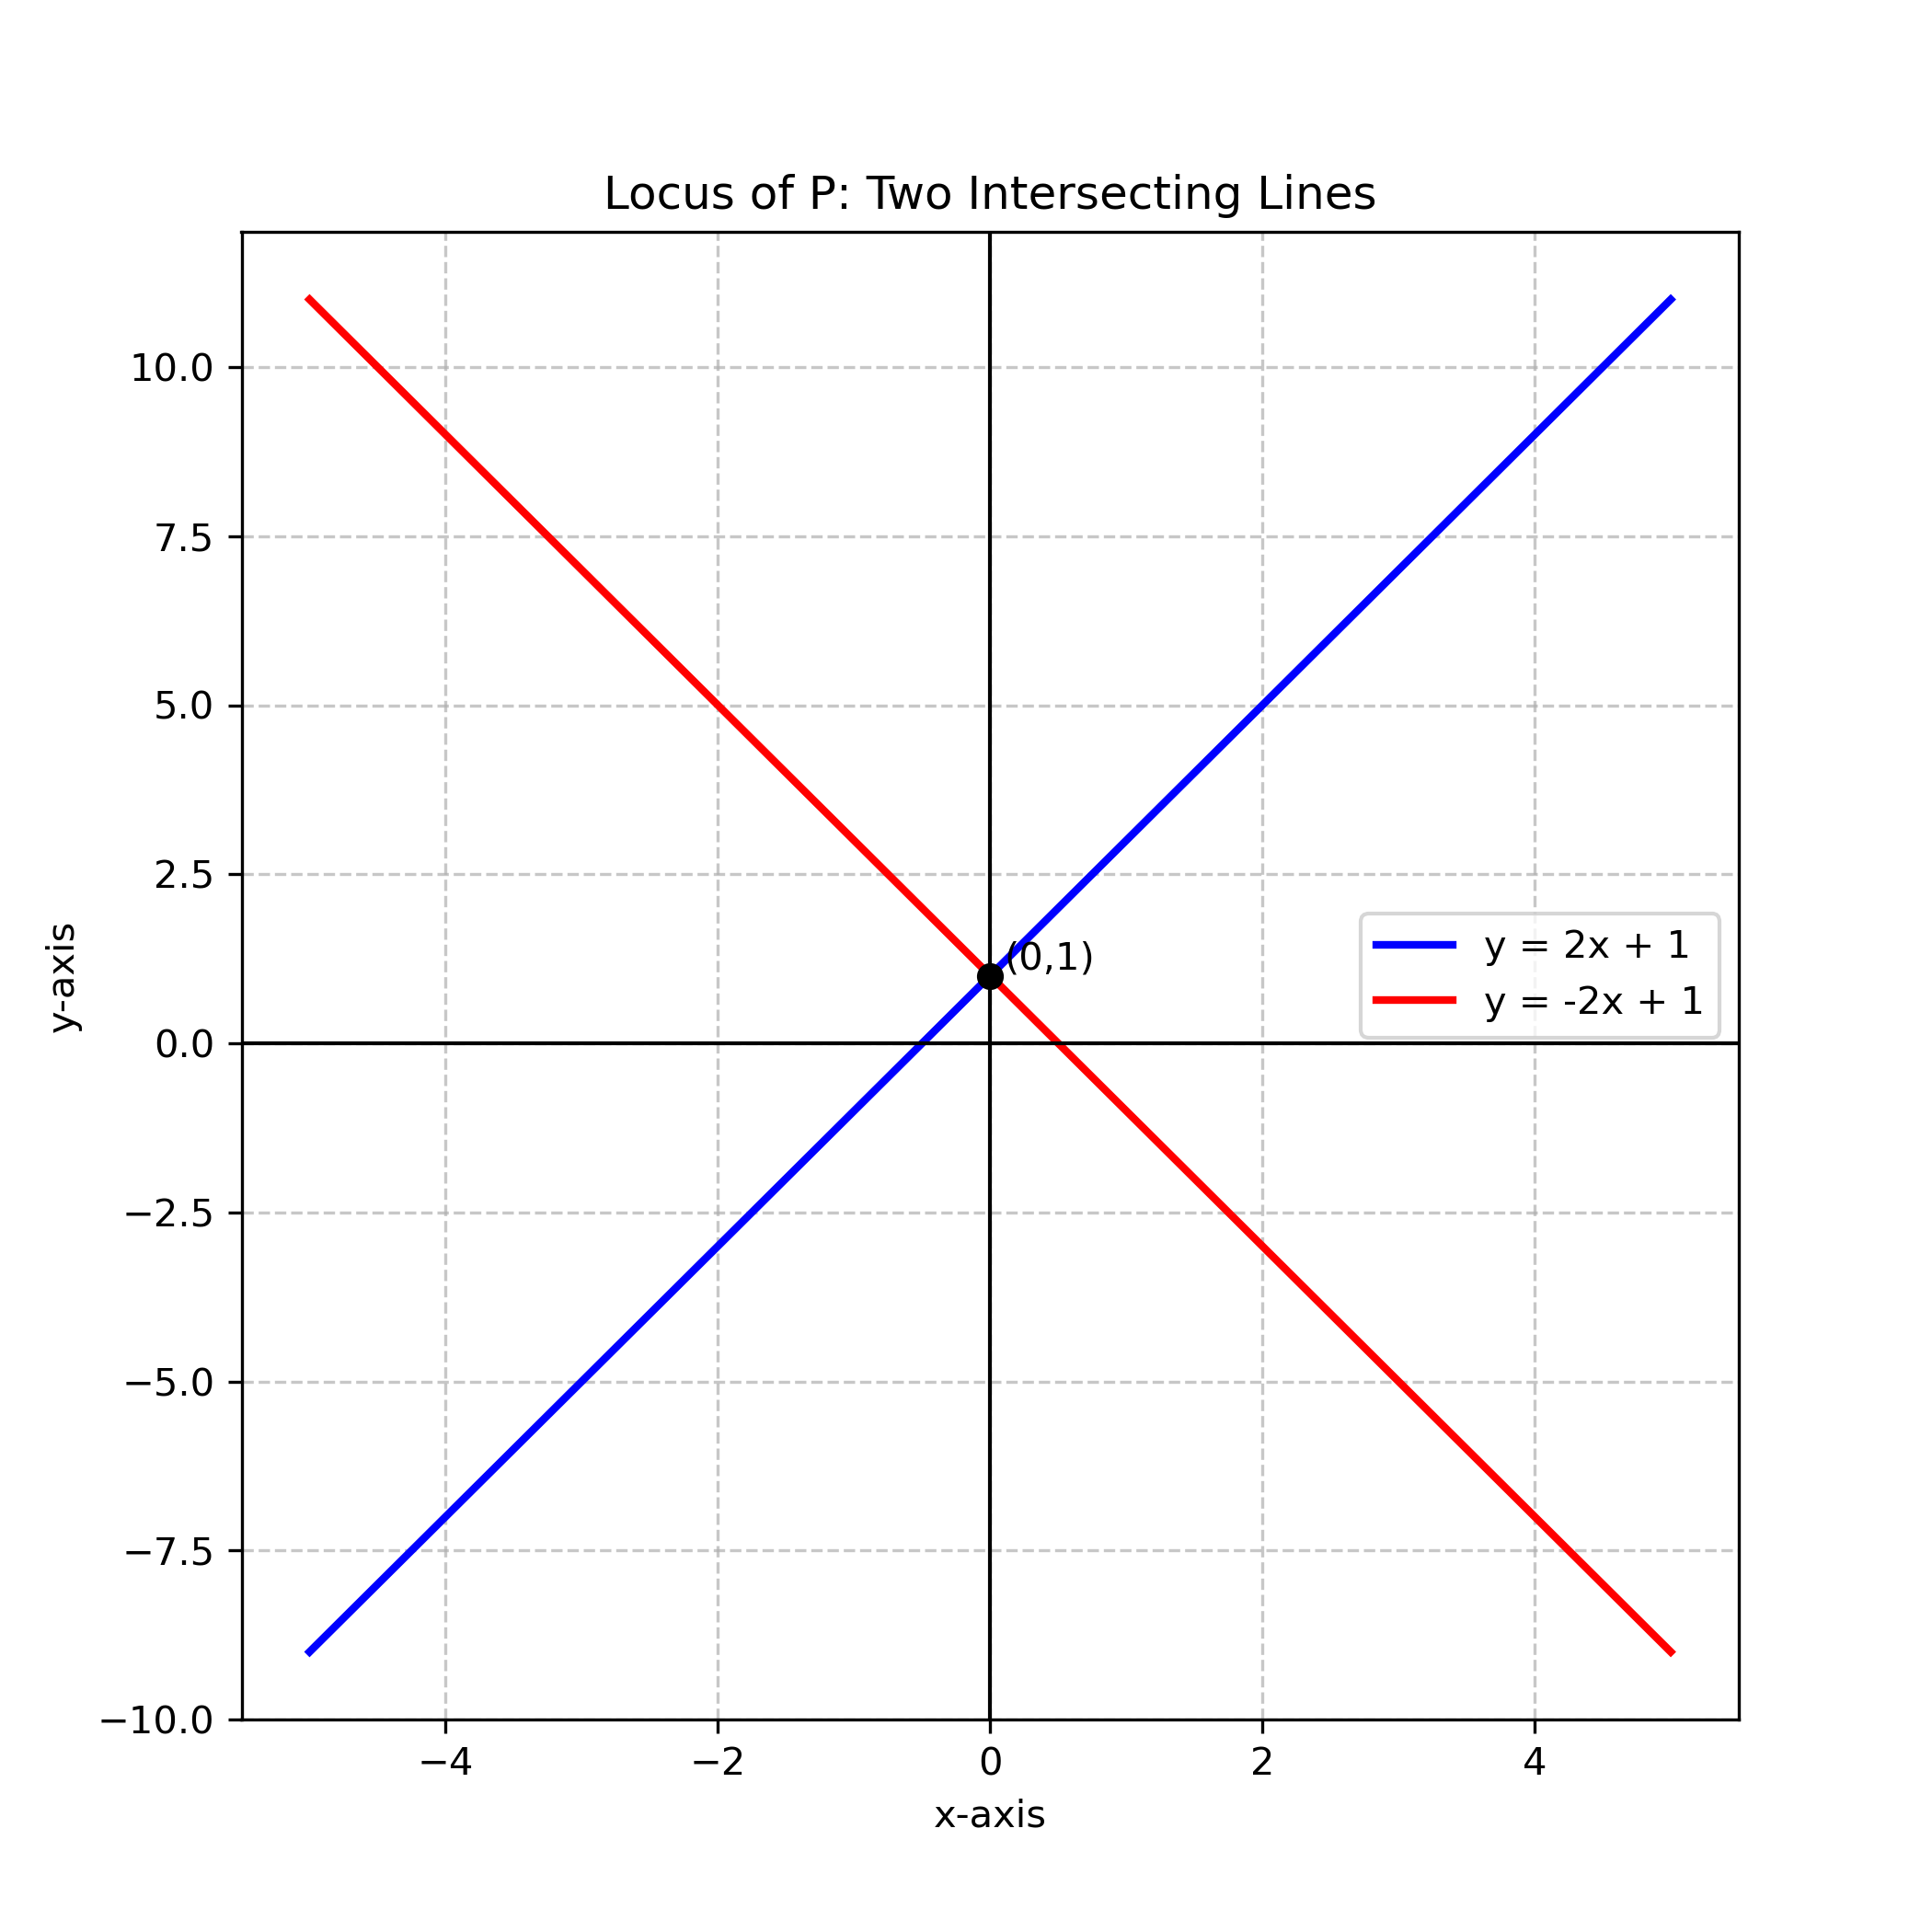
\includegraphics[width=0.96\columnwidth]{figs/01.png}
    \label{fig-1}
\end{figure}
\end{document}
